%%%%%%%%%%%%%%%%%%%%%%%%%%%%%%%%%%%%%%%%%%%%%%%%%%%%%%%%%%%%%%%%%%%%%%%%%%%%%%%%%%%%%%
% Template fuer Abschlussarbeiten von Studierenden der 
% Frankfurt University of Applied Sciences
% 
% erstellt von: Prof. Dr.-Ing. Thomas Hollstein
% 
% Last revision: 22.06.2023
%
%%%%%%%%%%%%%%%%%%%%%%%%%%%%%%%%%%%%%%%%%%%%%%%%%%%%%%%%%%%%%%%%%%%%%%%%%%%%%%%%%%%%%%


\documentclass[
    %twoside, 
    %openright,
  titlepage,
  numbers=noenddot,
  headinclude,
    %1headlines,
  footinclude=true,
    %cleardoublepage=empty,
    %BCOR=5mm,
  fontsize=20pt,%20pt,
  paper=a4,
    %letterpaper
    %a4paper,
  ngerman,
  american,
    %table
  ]
% Dokumententyp: (legt grundlegende Formatierrichtlinien fest)
    %{book}
    %{report}
{report}
    %{scrreprt}

%%%%%%%%%%%%%%%%%%%%%%%%%%%%%%%%%%%%%%%%%%%%%%%%%%%%%%%%%%%%%%%%%%%%%%%%%%%%%%%%%%%%%%


   

% Farbigen Text
\usepackage{xcolor}

\parindent = 0pt  % Neue Absaetze nicht einruecken
\parskip = 1ex % Neue Absaetze: 1/2 Zeile Abstand





%%%%%%%%%% zu nutzende Pakete einbinden: %%%%%%%%%%

%%%%% Package Kommentare:



\usepackage{comment}
\usepackage[colorinlistoftodos]{todonotes}
\newcommand{\mycomment}[1]{\todo[inline,linecolor=green,backgroundcolor=yellow!25,bordercolor=green,caption={}]{todo: #1}}



%%%%% package Sprachunterstuetzung:

\usepackage{babel}[ngerman]
\usepackage{minted}
\usepackage{csquotes}

%%%%% Package Multirow ermoeglicht, dass sich ein Kaestchen in einer Tabelle ueber mehrere Zeilen erstrecken kann:

\usepackage{multirow}

% Beispiele unter: https://texblog.org/2012/12/21/multi-column-and-multi-row-cells-in-latex-tables/

%Vereinigung von Feldern in Tabellen:
%\multicolumn{number cols}{align}{text} % align: l,c,r
%\multirow{number rows}{width}{text}

%%%% Serifenloser Textstil fuer das ganze Dokument: 

\RequirePackage[sfdefault,lf]{carlito}
\usepackage{lmodern}
% \RequirePackage[T1]{fontenc}
% to imitate Calibri:
\renewcommand*\familydefault{\sfdefault} %% Base font of the document is to be sans serif

%%%%%% Grafiken einbinden
\usepackage{graphicx}
% https://golatex.de//wiki/%5cincludegraphics

%%%%%% Mathematik-Paket AMSMath:
\usepackage[fleqn,reqno]{amsmath}

\usepackage{setspace}


%%%%%% Seitengeometrie einstellen:
% https://tex.stackexchange.com/questions/344241/logo-as-header-using-fancyhdr-package
\usepackage{geometry}
\geometry{verbose,
          bmargin=2.5cm,
          lmargin=2cm,
          rmargin=2cm
          %footskip=-25pt
          }

%%%%%% die Höhe des Top-Margin errechnen:
\newlength\mytopmargin
\newsavebox{\headbox}\savebox{\headbox}{
    %\includegraphics[width=0.3\textwidth]{Figures/xxx.png} \hfill
    \raisebox{-1ex}{
\includegraphics[width=0.1\textwidth]{Figures/fra-uas_logo.pdf}}
}    
\setlength{\mytopmargin}{\totalheightof{\usebox{\headbox}}+2cm}
\geometry{verbose,
          tmargin=\mytopmargin,
          headheight=1.1\mytopmargin,
          footskip=9ex
}

% Flexiblere Tabellen
\usepackage{tabularx}
\def\tabularxcolumn#1{m{#1}}

% Boxen für Lickert Skalen
\usepackage{wasysym}
\newcommand\insq[1]{%
    \Square\ #1\quad%
}

% Durchstreichen von Text
\usepackage[normalem]{ulem} % mit \sout



%%%%%% Gesamtseitenzahl verwenden:
\usepackage{totpages}

%%%%%% Kalkulationen:
%https://tex.stackexchange.com/questions/30081/how-can-i-sum-two-values-and-store-the-result-in-other-variable
\usepackage{tikz}
\usetikzlibrary{math}

%%%%%% Gestaltung von Kopf- und Fusszeilen:
% https://tex.stackexchange.com/questions/344241/logo-as-header-using-fancyhdr-package
\usepackage{fancyhdr}
\pagestyle{fancy}  % Eigener Seitenstil
\fancyhf{}         % Alle Kopf- und Fußzeilenfelder bereinigen
%\fancyhead[L]{} % Kopfzeile links
\fancyhead[l]{\leftmark
   %\makebox[0.3\textwidth]{\includegraphics[width=0.3\textwidth]{Figures/xxx.png}}
}  
\fancyhead[c]{\hspace*{0.15\textwidth}\rightmark}
%\fancyhead[C]{\usebox\headbox}                        % Zentrierte Kopfzeile
\fancyhead[R]{
  \makebox[0.2\textwidth]{\raisebox{-1ex}{\hspace*{14ex}
\includegraphics[width=0.1\textwidth]{Figures/fra-uas_logo.pdf}}}
}  % Kopfzeile rechts
\renewcommand{\headrulewidth}{0.4pt} % Obere Trennlinie
%\fancyfoot[L]{\today}
\fancyfoot[C]{\ThesisTitleShort} 
%\fancyfoot[R]{Seite \thepage ~von \ref{TotPages}}  % Seitennummer
\fancyfoot[R]{\thepage} % Seitennummer 
\renewcommand{\footrulewidth}{0.4pt} % Untere Trennlinie
\setlength{\mytopmargin}{\totalheightof{\usebox\headbox} +2cm}
%Unterschied zwischen geraden/ungeraden Seiten:
%\fancyhead[OR]{} % "O" steht für "odd", also ungerade Seiten
%\fancyhead[ER]{} % "E" für "even", also gerade Seiten.




%%%%% Erweiterte Formate für Listen/Aufzaehlungen:
\usepackage{paralist}
%Default-Items fuer die vier moeglichen Verschachtelungsebenen:
\setdefaultitem{}{\textbullet}{$\star$}{}

%%%%% FRA-UAS CI Farben:
%\definecolor{airforceblue}{rgb}{0.36, 0.54, 0.66}
% CI-Farben FRA-UAS (blau):
\definecolor{FRAUAS_Blue_Dark}{RGB}{45, 137, 204}
\definecolor{FRAUAS_Blue_Light}{RGB}{182, 210, 228}
% CI-Farben FRA-UAS: FB1
\definecolor{FRAUAS_FB1_Dark}{RGB}{124, 128, 52}
\definecolor{FRAUAS_FB1_Light}{RGB}{213, 213, 179}
% CI-Farben FRA-UAS: FB2
\definecolor{FRAUAS_FB2_Dark}{RGB}{255, 158, 27}
\definecolor{FRAUAS_FB2_Light}{RGB}{251, 221, 173}
% CI-Farben FRA-UAS: FB3
\definecolor{FRAUAS_FB3_Dark}{RGB}{196, 213, 42}
\definecolor{FRAUAS_FB3_Light}{RGB}{237, 240, 166}
% CI-Farben FRA-UAS: FB4
\definecolor{FRAUAS_FB4_Dark}{RGB}{204, 31, 47}
\definecolor{FRAUAS_FB4_Light}{RGB}{240, 166, 183}

%%%%% Sektionstitel nach CI-Farben einfärben:
\usepackage{titlesec}
\titleformat{\section}
{\color{FRAUAS_Blue_Dark}\normalfont\Large\bfseries} %Titel
{\color{FRAUAS_Blue_Dark}\thesection}{1em}{}
\titleformat{\subsection}
{\color{FRAUAS_Blue_Dark}\normalfont\large\bfseries} %Titel
{\color{FRAUAS_Blue_Dark}\thesubsection}{1em}{}

%\usepackage{appendix}

%%%%% Erweiterte Bibliographie-Stile:
%\usepackage{harvard}
% Title Page
% (wir generieren den Titel per Handlayout und verwenden
% daher die folgenden Befehle nicht)
%\title{}
%\author{}

% https://www.overleaf.com/learn/latex/Hyperlinks
\usepackage{hyperref}
\hypersetup{
    %hyperindex=true,
    %linktocpage=true, % Seitenzahl statt Titel verlinkt
    colorlinks=true,
    linkcolor=black,
    filecolor=black,      
    urlcolor=black,
    pdftitle={Thesis},
    pdfpagemode=FullScreen,
    citecolor=black,
    }



%\usepackage[hyphens]{url}  %% stellt \url{} zur Verfuegung

%%%%% modernes BibLaTeX mit biber %%%%%
% https://golatex.de/viewtopic.php?t=13917
%\usepackage[style=ieee-alphabetic,
%backend=biber, natbib=true]{biblatex}

% Literatur nach Erscheinen im Text sortiert
%\usepackage[sorting=none, style=numeric,backend=biber, natbib=true]{biblatex}
%\usepackage[style=apa, backend=biber, natbib=true, sorting=nyt, sortcites=false]{biblatex}
\usepackage[style=numeric, backend=biber, natbib=true, sorting=none, sortcites=false]{biblatex}
% Ohne eingestellte Sortierung
%\usepackage[ style=numeric,
%backend=biber, natbib=true]{biblatex}


\addbibresource{bibliography.bib}

% Immer shortautor anzeigen, falls vorhanden
\makeatletter
\def\cbx@apa@ifnamesaved{\@firstoftwo}
\makeatother

% Zeilenabstand für das ganze Dokument (1.0 = Normalwert):
\renewcommand{\baselinestretch}{1.0}

\usepackage{fontsize}
  \changefontsize[14]{14}

\usepackage[acronym]{glossaries}
\makeglossaries

\usepackage{siunitx}

%%%%%%%%%%%%%%%%%%%%%%%%%%%%%%%%%%%%%%%%%%%%
%%%%% hier beginnt das eigentliche Dokument 
%%%%%%%%%%%%%%%%%%%%%%%%%%%%%%%%%%%%%%%%%%%%


\begin{document}

%%%%% Settings einbinden:
\newcommand{\myName}{Luca Andrea John Vinciguerra}
\newcommand{\ThesisTitle}{Nebenläufige Algorithmen im maschinellen Lernen: Analyse,
Implementierung und vergleichende Untersuchungen zur Parallelisierung
einer Bibliothek für künstliche neuronale Netze}
\newcommand{\ThesisTitleShort}{Nebenläufige Algorithmen im maschinellen Lernen}
%\newcommand{\ThesisSubtitle}{This is the subtitle of the thesis}
\newcommand{\ThesisDegree}{Bachelor of Science (B.Sc.)} 
%\newcommand{\ThesisDegree}{Bachelor of Arts (B.A.)}
%\newcommand{\ThesisDegree}{Master of Science (M.Sc.)}
%\newcommand{\ThesisDegree}{Master of Arts (M.A.)}
\newcommand{\myStudentId}{1296334}
\newcommand{\Supervisor}{Prof. Dr. Thomas Gabel}
\newcommand{\CoSupervisor}{Prof. Dr. Christian Baun}
\newcommand{\Faculty}{Fachbereich 2: Informatik und Ingenieurwissenschaften}
\newcommand{\University}{Frankfurt University of Applied Sciences}
\newcommand{\UniversityLocation}{Frankfurt}
\newcommand{\ThesisDeliveryDate}{21. Mai 2023}
\newcommand{\CompanyName}{NoCompanyInvolved}  % don't modify this line, if no company is involved


%%%%%%%%%%%%%%%%%%%%% FOR ENGLISH LANGUAGE THESIS: %%%%%%%%%%%%%%%%%%%%

% By default the thesis language is german
% if you want to set it to ENGLISH, then UNCOMMENT the FOLLOWING LINE by removing the leading "%":

%\newcommand*{\ThesisLanguageIsEnglish}{}


\sloppy %Formatierungsueberstaende am Zeilenende vermeiden
% https://latexref.xyz/_005cfussy-_0026-_005csloppy.html

\frenchspacing  
%Ein Leerzeichen nach Satzende
%https://texwelt.de/fragen/1154/was-ist-french-spacing-was-macht-frenchspacing

%\raggedbottom   
%Standard is \flushbottom, dass heisst
%alle Seiten werden so gedehnt, dass sie 
%gleich hoch sind 
%Schaltet man \raggedbottom ein, ist dies
%nicht so

\ifdefined\ThesisLanguageIsEnglish
\selectlanguage{american}
\else
\selectlanguage{ngerman} % ngerman, american
\fi
%Deutsch nach neuer Rechtschreibung als
%Standardsprache fuer das Dokument einstellen

%\renewcommand*{\bibname}{new name}
%\setbibpreamble{}

% Numerierungstiefe setzen:
% 2: bis subsection (Standard)
% 3: bis subsubsection
\setcounter{secnumdepth}{3} %setzt die Numerierungstiefe



%\renewcommand{\thepage}{\Roman{page}}
\pagestyle{plain} % Seite ohne Kopf- und Fusszeilen darstellen



% hier wird die Titelseite eingebunden:
\thispagestyle{empty}
%\pdfbookmark[0]{Titelblatt}{title}

%*******************************************************
% Titlepage
%*******************************************************
%%%
%%% title page (german)
%%%
\thispagestyle{empty}
\pdfbookmark[0]{Titelblatt}{title}
\begin{titlepage}


  \vspace*{-3,5cm}
  \begin{center}
    
\includegraphics[width=7.7cm]{Figures/fra-uas_logo} \\ 
  \end{center}

  \begin{center}
    \vspace{0.1cm}
    \LARGE \textbf{Frankfurt University\\ of Applied Sciences}\\
    \vspace{0.4cm}
    \Large -- \Faculty --
  \end{center}

  \vfill

  \begin{center}
    \huge \textbf{\ThesisTitle}   %%%%% >>>>> Bitte in TeXFiles/000_Settings eintragen 
  \end{center} 

  \vfill

  \ifdefined\ThesisLanguageIsEnglish 
  \begin{center}
    \Large Thesis submitted in order to obtain the academic degree\\
    \vspace{0.3cm}
    \Large \ThesisDegree   %%%%% >>>>> Bitte in TeXFiles/000_Settings eintragen 
  \end{center}
  \else
  \begin{center}
    \Large Abschlussarbeit zur Erlangung des akademischen Grades\\
    \vspace{0.3cm}
    \Large \ThesisDegree   %%%%% >>>>> Bitte in TeXFiles/000_Settings eintragen 
  \end{center}
  \fi

  \vfill

  \ifdefined\ThesisLanguageIsEnglish 
  \begin{center}
    \Large submitted on \ThesisDeliveryDate\ on\\   %%%%% >>>>> Bitte in TeXFiles/000_Settings eintragen
    \vspace{0.3cm}
    \Large \textbf{\myName}\\
    \vspace{0.3cm}
    \normalsize Student ID: \myStudentId   %%%%% >>>>> Bitte in TeXFiles/000_Settings eintragen
  \end{center}
  \else
  \begin{center}
    \Large vorgelegt am \ThesisDeliveryDate\ von\\   %%%%% >>>>> Bitte in TeXFiles/000_Settings eintragen
    \vspace{0.3cm}
    \Large \textbf{\myName}\\
    \vspace{0.3cm}
    \normalsize Matrikelnummer: \myStudentId   %%%%% >>>>> Bitte in TeXFiles/000_Settings eintragen
  \end{center}
  \fi

  \vfill

  \ifdefined\ThesisLanguageIsEnglish 
  \begin{center}
    \begin{tabular}{lll}
      First Supervisor    & : & \Supervisor \\     %%%%% >>>>> Bitte in TeXFiles/000_Settings eintragen
      Second Supervisor & : & \CoSupervisor\\    %%%%% >>>>> Bitte in TeXFiles/000_Settings eintragen
    \end{tabular}
  \end{center} 
  \else
  \begin{center}
    \begin{tabular}{lll}
      Referent    & : & \Supervisor \\     %%%%% >>>>> Bitte in TeXFiles/000_Settings eintragen
      Korreferent & : & \CoSupervisor\\    %%%%% >>>>> Bitte in TeXFiles/000_Settings eintragen
    \end{tabular}
  \end{center} 
  \fi

\newpage


  

\end{titlepage}

%*******************************************************
% Non Disclosure Notice
%*******************************************************

\ifdefstring{\CompanyName}{NoCompanyInvolved}{}{
\ifdefined\ThesisLanguageIsEnglish
\chapter*{Non-Disclosure Notice}
\thispagestyle{empty}
This scientific thesis contains information of the company \CompanyName. The disclosure or
unauthorized use of this thesis as a whole or in parts is prohibited. The prohibition shall only
apply to information pertaining to the company \CompanyName. Any other exceptions require the
written consent of \CompanyName.
\medskip
\else
\chapter*{Sperrvermerk}
\thispagestyle{empty}
Die Vorliegende Arbeit beinhaltet vertrauliche Informationen des Unternehmens \CompanyName. 
Die Weitergabe oder Verwendung der Arbeit oder einzelner Informationen daraus ist in jeglicher
Form untersagt. Dieses Verbot gilt nicht für Informationen, die weder aus dem Unternehmen \CompanyName\ stammen noch diese betreffen. Sonstige Ausnahmen bedürfen der schriftlichen
Genehmigung des Unternehmens \CompanyName.
\medskip
\fi

}



%*******************************************************
% Declaration
%*******************************************************

\ifdefined\ThesisLanguageIsEnglish
\chapter*{Declaration}
\thispagestyle{empty}

Hereby I assure that I have written the presented thesis independently and without any third party help and that I have not used any other tools or resources than the ones mentioned/referred to in the thesis.
\medskip

\noindent
Any parts of the thesis that have been taken from other published or yet unpublished works in terms of their wording or meaning are thoroughly marked with an indication of the source. 
\medskip

\noindent
All figures in this thesis have been drawn by myself or are clearly attributed with a reference. 
\medskip

\noindent
This work has not been published or presented to any other examination authority before.
I am aware of the importance of the affidavit and the consequences under examination
law as well as the criminal consequences of an incorrect or incomplete affidavit.
\medskip


\else
\chapter*{Eidesstattliche Erklärung}
\thispagestyle{empty}
Ich versichere hiermit, dass ich die vorliegende Arbeit selbständig verfasst und keine anderen als die im Literaturverzeichnis angegebenen Quellen benutzt habe.
\medskip

\noindent
Alle Stellen, die wörtlich oder sinngemäß aus veröffentlichten oder noch nicht veröffentlichten Quellen entnommen sind, sind als solche kenntlich gemacht.
\medskip

\noindent
Die Zeichnungen oder Abbildungen in dieser Arbeit sind von mir selbst erstellt worden oder mit einem entsprechenden Quellennachweis versehen.
\medskip

\noindent
Diese Arbeit ist in gleicher oder ähnlicher Form noch bei keiner anderen Prüfungsbehörde eingereicht worden. 
\bigskip
\fi

Frankfurt am Main, \ThesisDeliveryDate

\smallskip


\hfill {\raisebox{-2ex}{
\includegraphics[width=5cm]{Figures/YourSignature_w.png}\ \ }} \\ 
\vspace*{-7ex}
\begin{flushright}
    \begin{tabular}{m{5cm}}
        \\ \hline
        \centering \textbf{\myName}\\
    \end{tabular}
\end{flushright}
%\textbf{\myName}
\newpage

% da wir den Titel haendisch erstellt haben entfaellt der folgende Befehl:
%\maketitle

%\clearpage

%\pagestyle{headings} 
\pagestyle{fancy}   % Seite mit Kopf- und Fusszeilen darstellen
\pagenumbering{roman}  % Umschalten auf Seitenzahlen in römischer Darstellung
%\fancyfoot[R]{i}  % Seitennummer
%roemisch 1, hier per Hand eingetragen, weil es anders nicht funktioniert hat - hat sich erledigt


\tableofcontents
\clearpage
\pagenumbering{arabic}  % Umschalten auf Seitenzahlen in arabischer Darstellung
%%%%% Einbinden der Dateien für die einzelnen Sektionen:
% Verwendet man hier \include statt \input, beginnen
% neue Sektionen immer auf einer neuen Seite
%\input{TeXFiles/Abstract}

\fancyfoot[R]{\thepage}  % Seitennummer

%\myName
\setstretch{1.5}
\ifdefined\ThesisLanguageIsEnglish
\chapter*{Abstract}
\else
\chapter*{Kurzfassung}
\fi
\label{ch:Abstract}


\chapter{Einleitung}
\label{ch:Einleitung}

Die Informatik schöpft oft Inspiration aus der Natur, sei es durch die Nachahmung tierischer Bewegungen bei Robotern, der Organisation von Multiagentensystemen in vogelähnlichen Schwärmen oder der Anwendung evolutionärer Algorithmen zur Simulation natürlicher Prozesse. Doch eines der faszinierendsten Phänomene der Natur ist das menschliche Gehirn und seine Fähigkeit, aus Erfahrung zu lernen. Dieses komplexe Organ beschäftigt Wissenschaftler seit langem, und die Suche nach Möglichkeiten, seine Lernfähigkeit zu simulieren, hat zu bedeutenden Fortschritten geführt.

Ein zentrales Element im Gehirn ist das Neuron, auch Nervenzelle genannt, das als Grundbaustein für die Informationsverarbeitung dient. Das Menschliche Gehirn besitzt circa 10 Milliarden Neuronen. Jedes dieser Neuronen besteht aus einem Zellkörper, mehreren Dendriten und einem Axon. Die Dendriten empfangen elektrische Signale von davor geschalteten Neuronen und fungieren somit als Eingangsebene für Informationen. Diese eingehenden Signale werden zum Zellkörper weitergeleitet, wo sie aufsummiert werden. Wird ein bestimmter Schwellenwert überschritten, leitet das Neuron das elektrische Potenziale über das Axon weiter, welches es elektrochemisch an nachgeschaltete Neuronen über deren Dendriten weiterleitet. Das Axon agiert somit als Ausgangsebene für Informationen des Neurons. 
Durch diese Kettenreaktion können im Gehirn somit komplexe Sachverhalte verarbeitet werden \citep{Praktische_Einfuhrung_in_neuronale_Netze}.

Inspiriert von diesem biologischen Vorbild entwickelte Frank Rosenblatt 1958 das Modell des Perzeptrons - ein künstliches Neuron, welches die Grundlage für die Entwicklung heutiger künstlicher neuronaler Netzwerke darstellt \citep{Rosenblatt_Perceptron}. Diese Netzwerke können mithilfe von Lernalgorithmen trainiert werden, um vielfältige Probleme zu bewältigen, welche mit konventionellen Computeralgorithmen, wenn überhaupt, nur schwer zu lösen sind. Mittlerweile tragen künstliche neuronale Netzwerke mitunter in verschiedensten Branchen zu der Realisierung von Software in vielfältigen Anwendungsgebieten bei.

Aufgrund der großen Menge an Daten und benötigten Rechenleistung für die Darstellung von neuronalen Netzwerken in Computern ist die Frage der Skalierbarkeit und Effizienz der neuronalen Netzwerke von entscheidender Bedeutung. Insbesondere die Verarbeitung großer Datenmengen erfordert effiziente Algorithmen und Techniken zur Parallelisierung, um den gegebenen Anforderungen beispielsweise im Bezug auf Latenz gerecht zu werden. In dieser Arbeit wird daher die Parallelisierung von neuronalen Netzen thematisiert und untersucht, wie diese Techniken die Leistung und Effizienz beeinflussen.

\section{Aufgabenstellung}
\label{sec:Einleitung_Aufgabenstellung}
In Anbetracht der stagnierenden Entwicklung der Taktrate aufgrund des Annäherns an das physikalische Limit konnten in den letzten Jahren keine großen Verbesserungen in der Einkernleistung erzielt werden. Deshalb setzten Prozessorhersteller weit verbreitet auf Mehrkernprozessoren, um Leistungssteigerungen zu ermöglichen \citep{Chip_makers_turn_to_multicore}. Angesichts der möglichen Leistungssteigerung durch effizientes Nutzen aller verfügbaren Kerne ist es von besonderem Interesse, die Leistung der bestehenden n++-Bibliothek für maschinelles Lernen durch Parallelisierung zu verbessern \citep{Riedmiller_RPROP}. Die n++-Bibliothek ist in C++ implementiert, weshalb die Parallelisierung mithilfe von Threads realisiert werden soll. Eine zentrale Herausforderung besteht darin, geeignete Stellen in der Bibliothek als auch in Anwendungsprogrammen zu identifizieren, die von der Parallelisierung profitieren könnten. Hierbei werden vorhandene Vorarbeiten \citep{thesis_Artur_Brening} und Implementierungen als Vergleich herangezogen und gegebenenfalls optimiert.

Diese Arbeit zielt darauf ab, die potenziell erzielten Leistungsverbesserungen durch die Parallelisierung zu untersuchen und zu quantifizieren. Durch die Implementierung der Parallelisierung und die anschließende Ausführung von Algorithmen der Vorarbeit kann der Effekt der Parallelisierung auf die Leistung von Programmen, welche die n++-Bibliothek verwenden, evaluiert werden. Zudem werden die Auswirkungen verschiedener Parameter und Konfigurationen im Zusammenhang mit der Parallelisierung analysiert, um ein umfassendes Verständnis der Leistungsverbesserung durch Parallelisierung zu erlangen.

Insgesamt strebt diese Arbeit danach, nicht nur die technische Umsetzung der Parallelisierung zu präsentieren, sondern auch deren Auswirkungen auf die Leistungsfähigkeit der n++-Bibliothek für maschinelles Lernen zu untersuchen und zu bewerten.

\section{Gliederung}
\label{sec:Einleitung_Gliederung}


Nach einer Einführung in die Thematik und die Vorgehensweise der Arbeit im ersten Kapitel, folgt im zweiten Kapitel die Vermittlung der notwendigen Grundlagen. Dazu gehören die Grundprinzipien neuronaler Netze sowie die Grundlagen der Parallelisierung.
Das dritte Kapitel beschreibt die Implementierung der Parallelisierung im n++-Simulator. Nach der Erläuterung des n++-Simulatorkerns und der Analyse des bestehenden Codes werden die Voraussetzungen für die Parallelisierung geschaffen und die Implementierung detailliert vorgestellt.
Im vierten Kapitel werden die experimentellen Untersuchungen zur Evaluation der Parallelisierungstechniken präsentiert. Die Testumgebung, die Testmethodik und die Ergebnisse der experimentellen Untersuchungen werden ausführlich beschrieben und analysisert.
Abschließend fasst das Fazit die wichtigsten Ergebnisse der Arbeit zusammen und gibt einen Ausblick auf mögliche Forschungsarbeiten.
\chapter{Grundlagen}
\label{ch:Grundlagen}

Das folgende Kapitel legt die Grundlagen für künstliche neuronale Netzwerke dar, indem es detailliert auf ihre Struktur und Funktionsweise eingeht, insbesondere für vorwärtsgerichtete Netzwerke. Dabei wird ein umfassender Überblick über die potenziellen Anwendungsbereiche von künstlichen neuronalen Netzwerken gegeben, wobei deren Rolle in verschiedenen Bereichen wie Bilderkennung, Sprachverarbeitung und Mustererkennung hervorgehoben wird.

Des Weiteren wird die Thematik der Parallelisierung sowohl im allgemeinen Kontext als auch speziell im Zusammenhang mit neuronalen Netzwerken erläutert. Es werden die Vor- und Nachteile dieser Technik beleuchtet und die gängigsten Methoden zur Parallelisierung von Berechnungen in neuronalen Netzwerken werden ausführlich diskutiert. Dabei wird besonders auf die Parallelisierung von Berechnungen innerhalb vorwärtsgerichteter Netzwerke eingegangen.

Die Nutzung von Grafikprozessoren (GPUs) für parallele Berechnungen wird dabei angesprochen, jedoch liegt der Fokus auf den grundlegenden Prinzipien der Parallelisierung von neuronalen Netzwerken und deren Implementierung mittels Thread- und Prozessparallelsierung. Durch das fundierte Verständnis der zugrunde liegenden Konzepte können wir die Potenziale und Herausforderungen der Parallelisierung in diesem spezifischen Kontext besser einschätzen und geeignete Ansätze zur Leistungssteigerung identifizieren.

\section{Grundprinzipien von neuronalen Netzwerken}
\label{sec:Grundlagen_neuronale_Netzwerke}

Neuronale Netzwerke sind ein wesentlicher Bestandteil des maschinellen Lernens und der künstlichen Intelligenz. Sie sind inspiriert von der Funktionsweise des menschlichen Gehirns und bestehen aus einer Ansammlung miteinander verbundener Knoten, die als Neuronen bezeichnet werden. Diese Netzwerke können eine Vielzahl von Aufgaben ausführen, von der Bilderkennung bis hin zur Sprachverarbeitung.

Die Funktionsweise eines neuronalen Netzwerks lässt sich grob in zwei Hauptphasen unterteilen: Vorwärtspropagierung und Rückwärtspropagierung. Während der Vorwärtspropagierung fließen die Daten durch das Netzwerk, beginnend mit den Eingangsneuronen, die die Rohdaten empfangen, und endend mit den Ausgangsneuronen, die die Vorhersagen oder Klassifikationen des Netzwerks liefern. Jedes Neuron in einem neuronalen Netzwerk ist mit anderen Neuronen verbunden, und diese Verbindungen sind mit Gewichten versehen, die die Stärke der Verbindung zwischen den Neuronen darstellen.

Während der Vorwärtspropagierung durchläuft jede Eingabe eine Reihe von Schichten im Netzwerk, wobei jede Schicht aus einer bestimmten Anzahl von Neuronen besteht. Jedes Neuron in einer Schicht erhält Inputs von den Neuronen der vorherigen Schicht, multipliziert diese Inputs mit den entsprechenden Gewichten und summiert sie. Anschließend wird eine Aktivierungsfunktion auf die gewichtete Summe angewendet, um die Ausgabe des Neurons zu berechnen, die dann an die Neuronen der nächsten Schicht weitergeleitet wird.

Die Rückwärtspropagierung ist der Prozess, bei dem das Netzwerk lernt, indem es seine Gewichte entsprechend der Fehler zwischen den tatsächlichen und den vorhergesagten Ausgaben anpasst. Dies geschieht durch die Berechnung von Gradienten mit Hilfe des Backpropagation-Algorithmus und die Anpassung der Gewichte mithilfe eines Optimierungsalgorithmus wie dem Gradientenabstiegsverfahren.

Insgesamt ermöglicht die Funktionsweise von neuronalen Netzwerken die Modellierung komplexer Zusammenhänge in Daten und die Durchführung verschiedenster Aufgaben des maschinellen Lernens und der künstlichen Intelligenz.

\section{Aufbau eines neuronalen Netzwerks}
\label{sec:Grundlagen_neuronale_Netzwerke}
\subsection{Neuronen und deren Verbindungen}
\label{sec:Grundlagen_neuronale_Netzwerke_Grundlagen}
\subsection{Schichten und ihre Funktionen}
\label{sec:Grundlagen_neuronale_Netzwerke_Aufbau}
\subsection{Vorwärtsgerichtete und rückwärtsgerichtete Netzwerke}
\label{sec:Grundlagen_neuronale_Netzwerke_Aufbau}

\section{Anwendungsfälle von neuronalen Netzwerken}
\label{sec:Grundlagen_neuronale_Netzwerke}

\section{Einführung in die Parallelisierung}
\label{sec:Grundlagen_neuronale_Netzwerke}
\subsection{Definition und Herangehensweise}
\label{sec:Grundlagen_neuronale_Netzwerke_Aufbau}
\subsection{Vor- und Nachteile von Parallelisierung}
\label{sec:Grundlagen_neuronale_Netzwerke_Aufbau}

\section{Parallelisierung in vorwärtsgerichteten Netzwerken}
\label{sec:Grundlagen_neuronale_Netzwerke}
\subsection{Thread- und Prozessparallelsierung}
\label{sec:Grundlagen_neuronale_Netzwerke_Aufbau}
\subsection{Implementierung von Parallelisierungstechniken}
\label{sec:Grundlagen_neuronale_Netzwerke_Aufbau}
\subsection{Auswirkungen auf die Leistungsfähigkeit}
\label{sec:Grundlagen_neuronale_Netzwerke_Aufbau}
\chapter{Implementierung der Parallelisierung}
\label{ch:Implementierung_Parallelisierung_Npp}
\chaptermark{Implementierung}

In diesem Kapitel wird zunächst die n++-Bibliothek und der bestehende Code vorgestellt, als auch auf den verwendeten Datensatz eingegangen. Anschließend werden die konzeptionellen Voraussetzungen erläutert und die Implementierung wird detailliert vorgestellt. Dabei wird auch die Struktur der neuen Implementierung mit der der Vorarbeit verglichen.

\section{Erläuterung des n++-Simulatorkerns}
\label{sec:Erlauterung_Npp}
\sectionmark{Erläuterung n++}
N++ ist ein Simulator für neuronale Netze, der als Forschungsprojekt an der Universität Karlsruhe entwickelt wurde. Die Software ermöglicht die Simulation mehrerer neuronaler Netze und strebt danach, dem Anwender eine einfache Erweiterung der Grundfunktionen sowie eine benutzerfreundliche Schnittstelle für Anwendungsprogramme bereitzustellen \citep{Riedmiller_RPROP}.

Die Bibliothek n++ ist in C++ verfasst. Da sie seit über 20 Jahren besteht, verwendet sie größtenteils keine modernen C++-Features, unter anderem auch um die Kompatibilität mit C beizubehalten, da der Kern des Simulators auf dieser älteren Sprachversion aufbaut. Oft werden im Quellcode Funktionen der Standardbibliothek von C denen von C++ vorgezogen.

N++ ermöglicht es dem Benutzer, die Topologie des neuronalen Netzes zu spezifizieren und es an die spezifischen Anforderungen anzupassen. Hierbei können Parameter wie die Anzahl der Schichten, die Größe der Schichten sowie die Dimensionen der Ein- und Ausgabeschichten festgelegt werden \citep{dokumentation_npp}. Nach der Konfiguration des Netzes können Eingabemuster durch Vorwärtspropagation propagiert werden. Die resultierenden Ausgaben können abgerufen werden, und optional kann durch Rückwärtspropagation des Fehlervektors ein Lernprozess des Netzwerks simuliert werden, wobei die Gewichte automatisch angepasst werden. Generierte Netze können in Dateien gespeichert werden, um sie zu einem späteren Zeitpunkt wiederzuverwenden, insbesondere für reproduzierbare Experimente.

In Codeausschnitt \ref{fig:npp_examplenet_code}, welcher eine vereinfachte Form des Beispielnetzes aus der n++-Dokumentation darstellt \citep{dokumentation_npp}, wird ein Beispielnetz mit drei Schichten erstellt. Die Eingabeschicht hat dabei zwei Parameter, die Ausgabeschicht drei, und die versteckte Schicht hat vier Parameter. Es ist ersichtlich, dass die n++-Bibliothek das einfache Austauschen von Updatefunktionen unterstützt. In den Zeilen 16 und 17 wird die Updatefunktion dynamisch auf Rückwärtspropagation gesetzt, was ohne großen Aufwand möglich ist.

\begin{figure}[H]
\begin{minted}
[
frame=lines,
framesep=2mm,
baselinestretch=1.2,
fontsize=\footnotesize,
linenos
]{c++}
#include "n++.h"

#define INPUTS 2
#define OUTPUTS 3
#define LAYERS 3

int main() {
    Net net;
    // Schichten des Netzes erstellen und miteinander verbinden
    int layerNodes[LAYERS] = {INPUTS, 4, OUTPUTS};
    net.create_layers(LAYERS, layerNodes);
    net.connect_layers();
    // Gewichte mit Zufallszahlen zwischen 0 und 0,5 initialisieren
    net.init_weights(0, 0.5);
    // Updatefunktion auf Rückwärtspropagation setzen
    float uparams[5] = {0.1, 0.9, 0, 0, 0};
    net.set_update_f(BP, uparams);
}
\end{minted}
\label{fig:npp_examplenet_code}
\caption{Vereinfachte Form des Beispielnetzes aus der n++-Dokumentation welche ein Netz mit 3 Schichten erstellt}
\end{figure}

\section{Bestehender Code}
\label{sec:Bestehender_Code_Brening}
\sectionmark{Bestehender Code}

Als bestehender Code wird ein Experiment aus der Bachelorarbeit von Artur Brening \citep{thesis_Artur_Brening} betrachtet. In dieser Bachelorarbeit wurde der Gradientenabstieg zum Trainieren neuronaler Netze implementiert. Dabei wurden viele Experimente mit verschiedenen Datensätzen und Lernmethoden zum Vergleich implementiert. Eines dieser Experimente wird als Grundlage für diese Bachelorarbeit übernommen.

Ausgewählt wurde das Experiment \enquote{MAGIC\_BP}, welches Rückwärtspropagierung nutzt. In dem Experiment wird der Magic Datensatz verwendet, auf welchen im nächsten Abschnitt eingegangen wird. Es wird ein mit Hilfe der n++-Bibliothek ein neuronales Netz erstellt und zunächst wird ein festgelegter Teil des Datensatzes als Trainingsdatensatz genommen, und jede dieser Trainingsdaten wird zunächst vorwärts durch das neuronale Netz propagiert. Anschließend wird der Fehler der resultierenden Ausgabe des Netzes bestimmt und es wird rückwärtspropagiert.
Nachdem alle Datensätze aus dem Trainingsdatensatz vor- und rückwärtspropagiert wurden, wird der verbleibende Teil des Datensatzes als Testdatensatz definiert. Genau wie die Trainingsdatensätze wird jeder Datensatz zuerst vor- und dann rückwärts propagiert. Nach jedem Datensatz wird hier jedoch geschaut, ob die Ausgabe des Netzes korrekt ist, um zu schauen, wie viele Daten des Testdatensatzes korrekt klassifiziert werden.
Dieser Prozess über den gesamten Datensatz wird für 10000 Epochen, also 10000 mal ausgeführt, um das Netz lernen zu lassen.

Dieser Lernprozess wird sequenziell für 10 verschiedene Netze mit 10 verschiedenen Startseeds ausgeführt, um das Verhalten mit verschiedenen Zufallszahlen zu überprüfen. Nachdem alle 10 Netze trainiert und getestet wurden, werden die Testergebnisse analysiert und in eine Datei geschrieben, um sie weiter verwerten zu können. Ein Durchlauf des bestehenden Programmes benötigt auf einem Apple M1 Pro Prozessor circa 1450 Sekunden.

\begin{figure}[H]
\centering
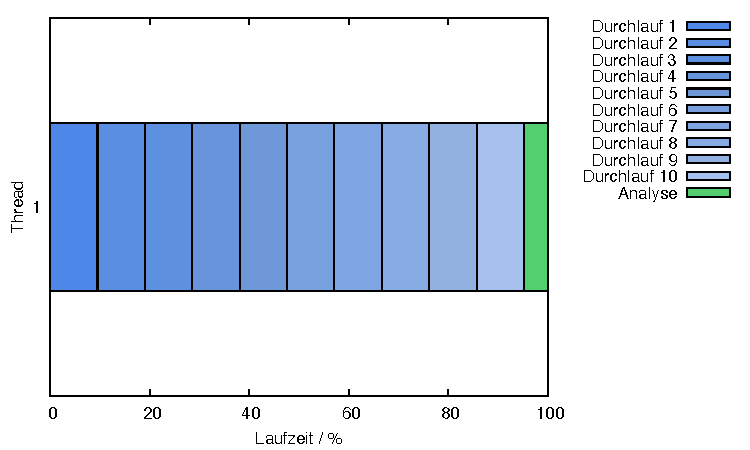
\includegraphics[width=0.8\textwidth]{../results/plots/timeline/timeline_plot_1thread.pdf}
\caption{Schematischer Ablauf des bestehenden Programms. In jedem Durchlauf wird ein neuronales Netz mit 10000 Epochen trainiert und anschließend getestet. In der Analyse werden die Ergebnisse aller Netze zusammengetragen und in eine Datei geschrieben.}
\label{fig:timeline_existing_code}
\end{figure}

Wie in Abbildung \ref{fig:timeline_existing_code} ersichtlich laufen alle Netze, auf der Grafik in blau dargestellt, auf einem Thread. Anschließend wird die Analyse, in grün dargestellt, ausgeführt. In dieser Arbeit werden die Trainings- und Testdurchläufe parallelisiert, was bedeutet, dass potenziell 10 Netze gleichzeitig trainiert und getestet werden können. Dies könnte möglicherweise zu großen Leistungsverbesserungen führen, da das Training und Testen der Netze den Großteil der Laufzeit einnimmt, und die Analyse nur wenige Sekunden in Anspruch nimmt. 

\section{Datensatz}
\label{sec:Datensatz}
\sectionmark{Datensatz}

Der verwendete Datensatz MAGIC Gamma Telescope aus dem UCI Machine Learning Repository ist eine bedeutende Ressource für die Forschung im Bereich der Gamma-Teleskopie. Er enthält eine Vielzahl von Beobachtungen, die von Gammastrahlen-Teleskopen gemacht wurden. Jede Beobachtung wird durch eine Reihe von Merkmalen beschrieben, die aus den gemessenen Eigenschaften der Gammastrahlen stammen. Das Hauptziel bei der Verwendung dieses Datensatzes ist die Klassifizierung von Beobachtungen in verschiedene Kategorien oder Klassen. Durch die Anwendung von Klassifizierungsalgorithmen können Muster und Zusammenhänge in den Daten identifiziert werden, was wiederum dazu beitragen kann, das Verständnis der Gammastrahlenphänomene im Universum zu vertiefen \citep{misc_magic_gamma_telescope_159}. Das UCI Machine Learning Repository ist eine bekannte Datenbank, die eine Vielzahl von Datensätzen für die Forschung und Entwicklung im Bereich des maschinellen Lernens bereitstellt. Die Daten sind kostenfrei verfügbar und können für verschiedene Zwecke verwendet werden. Der Datensatz enthält insgesamt 19020 Beobachtungen \citep{misc_magic_gamma_telescope_159}.

\section{Voraussetzungen}
\label{sec:Voraussetzungen_Parallelisierung}
\sectionmark{Voraussetzungen}
Für eine erfolgreiche Parallelisierung des Anwendercodes ist eine umfassende Analyse und Modifikation desselben unerlässlich. Dieser Abschnitt diskutiert die grundlegenden Voraussetzungen, die vor der Implementierung von Parallelisierungsstrategien berücksichtigt werden müssen. In erster Linie erfordert die Parallelisierung die Identifizierung und Beseitigung von Abhängigkeiten innerhalb des Algorithmus sowie die Anpassung der Implementierung, um die Effizienz und Skalierbarkeit auf mehreren Prozessoren oder Rechenkernen zu gewährleisten \citep{wilkinson2006parallel}.

\subsection{Entfernung von geteilten Speicherzugriffen}
\label{sec:Entfernung_geteilte_Speicherzugriffe}
Geteilte Speicherzugriffe, auch Shared Memory genannt, häufig realisiert durch globale Variablen im Quellcode, ermöglichen es verschiedenen Teilen eines Programms, auf dieselben Daten zuzugreifen. Diese Abhängigkeit ermöglicht es dem Programmierer komplexe Algorithmen simpel zu implementieren. Während dies in einer sequenziellen Umgebung einigermaßen gut funktionieren kann, können Probleme auftreten, wenn versucht wird, solche Konstrukte in einem parallelen Kontext zu verwenden.

Bei der Parallelisierung eines Programms ist es entscheidend, dass verschiedene Threads oder Prozesse unabhängig voneinander arbeiten können, um eine effiziente und sichere Ausführung zu gewährleisten. Globale Variablen führen jedoch schnell zu potenziellen Konflikten, da mehrere Threads gleichzeitig auf den gleichen Speicherbereich zugreifen können. Dies kann zu Wettlaufsituationen, inkonsistenten Zuständen und anderen unerwarteten Verhaltensweisen führen, die die Zuverlässigkeit und Korrektheit des Programms beeinträchtigen \citep{Czech_2017_Shared_Memory}.

Um dieses Problem zu lösen, ist es notwendig, die Abhängigkeit von geteilten Speicherzugriffen soweit wie möglich zu reduzieren. Dies erfolgt durch die Umstrukturierung des Quellcodes, um den Einsatz globaler Variablen zu minimieren oder ganz zu eliminieren. Statt globaler Variablen können lokale Variablen verwendet werden, die nur innerhalb bestimmter Funktionsbereiche gültig sind und somit den Zugriff auf den Speicher einschränken. Diese Vorgehensweise kann zusätzlich Vorteile im Bezug auf Speicherlecks und Speicherbedarf mit sich bringen, da die Variablen nur für die Zeit ihrer Verwendung gespeichert werden. Darüber hinaus können Datenstrukturen wie Klassen oder Strukturen verwendet werden, um Daten zu kapseln und den Zugriff über klar definierte Schnittstellen zu ermöglichen \citep{Czech_2017_Shared_Memory}.

Bei der Entfernung von geteilten Speicherzugriffen ist es wichtig, auch geeignete Synchronisationsmechanismen einzuführen, um kritische Abschnitte des Codes zu schützen. Dies kann die Verwendung von Mutexen, Semaphoren oder anderen Mechanismen umfassen, um sicherzustellen, dass nur ein Thread gleichzeitig auf bestimmte Ressourcen zugreifen kann, und so potenzielle Wettlaufbedingungen zu vermeiden. Die Verwendung von Mutexen sollte jedoch nicht ohne Vorbehalt in Erwägung gezogen werden, da sie weitere Abhängigkeiten schafft, welche die Leistungsgewinne durch mehrere Threads wieder negieren könnten. Ist dies der Fall, sollte über eine größere Umstrukturierung der Architektur nachgedacht werden, um das Programm mit Parallelisierung kompatibel zu machen \citep{Czech_2017_Shared_Memory}.

\subsection{Verlagerung der zu parallelisierenden Routine}
\label{sec:Verlagerung_parallelisierende_Routine}
Um eine effektive Parallelisierung zu erreichen, ist es von entscheidender Bedeutung, den spezifischen Teil des Codes zu identifizieren, der für die parallele Ausführung geeignet ist. Dieser Prozess erfordert eine sorgfältige Analyse des Quellcodes, um Bereiche zu lokalisieren, die unabhängig voneinander ausgeführt werden können und keine oder nur minimale Abhängigkeiten zu anderen Teilen des Programms aufweisen. Solche Bereiche können typischerweise Schleifen oder Abschnitte sein, die große Mengen von Daten verarbeiten, ohne auf Zwischenergebnisse anderer Bereiche angewiesen zu sein. Gegebenenfalls kann es auch sinnvoll sein, mit einem Profiler die Laufzeit des Programms zu analysieren, um zutreffende Teile zu identifizieren \citep{wilkinson2006parallel}.

Nachdem der geeignete Bereich identifiziert wurde, ist es notwendig, ihn aus dem Hauptcode auszulagern und in eine separate Routine oder Funktion zu überführen. Diese ausgelagerte Routine sollte autonom arbeiten können, ohne auf globale Variablen oder gemeinsam genutzte Ressourcen außerhalb ihres Bereichs zuzugreifen. Durch diese Isolierung können potenzielle Konflikte vermieden und die Parallelisierung erleichtert werden \citep{wilkinson2006parallel}.

Es ist essenziell sicherzustellen, dass die ausgelagerte Routine keine Abhängigkeiten zu anderen Teilen des Codes hat, um eine effiziente Parallelisierung zu ermöglichen. Hierbei müssen gegebenenfalls erforderliche Parameter übergeben und Rückgabewerte behandelt werden, um eine reibungslose Interaktion mit dem Rest des Programms zu gewährleisten \citep{wilkinson2006parallel}.

Die Verlagerung der zu parallelisierenden Routine ist mitunter der wichtigste Schritt bei der Implementierung von Parallelisierungsstrategien und bildet die Grundlage für eine effiziente und robuste parallele Ausführung des Programms. Durch die Identifizierung und Isolierung geeigneter Bereiche können potenzielle Engpässe reduziert und die Leistung des Programms optimiert werden.

Unter Umständen ist es nicht ohne Weiteres möglich, einfach einen bestimmten Teil des bestehenden Quellcodes auszulagern, und diesen zu parallelisieren. Ist dies der Fall, so muss der Quellcode allgemein konzeptionell umstrukturiert werden. In der Praxis ist dies einer der größten Faktoren, welche zu der Komplexität von Parallelisierung beitragen.

\section{Vorstellung der Implementierung}
\label{sec:Vorstellung_Implementierung}

In dieser Sektion wird genauer auf einige Aspekte der Implementierung eingegangen. Dabei werden auch einige Code-Ausschnitte behandelt, um die Änderungen und Implementierung zu veranschaulichen. 


\subsection{Verwendung von threadsicheren Funktionen}
\label{sec:Verwendung_threadsichere_Funktionen}

Besonders zur Manipulation von Zeichenketten macht sowohl die n++-Bibliothek als auch der Code des Experimentes von Herr Brening viel von klassischen Funktionen aus der C-Standardbibliothek gebrauch. Beispielsweise wird wie in Abbildung \ref{fig:strtok_usage_before} zu sehen in der n++-Bibliothek die Funktion strtok() verwendet, welche eine Zeichenkette tokenisieren kann, um ein neuronales Netz aus einer Datei zu laden und zu deserialisieren. 

\begin{figure}[H]
\begin{minted}
    [
    frame=lines,
    framesep=2mm,
    baselinestretch=1.2,
    fontsize=\footnotesize,
    linenos,
    firstnumber=611
    ]
    {c++}
int Net::load_net( char filename[] ) {
    ...
    else if (strncmp(line,"topology",7)==0){
        value=strtok(line, " \t\n");  /* skip first token (== topology)*/
        for(i=0,value=strtok( NULL," \t" );(value!=NULL)&&(i<MAX_LAYERS);
        value=strtok( NULL," \t\n" ),i++){
    ...
\end{minted}
\label{fig:strtok_usage_before}
\end{figure}

Werden mehrere Netze gleichzeitig geladen, kann die Verwendung von strtok() in diesem Kontext jedoch zu Problemen und Konflikten führen, da die strtok() Funktion intern den Zustand der Zeichenkettenzerteilung speichert, um bei folgenden Aufrufen den nächsten Teil der Zeichenkette zurückzugeben. Wenn die Funktion also an mehreren Stellen gleichzeitig aufgerufen wird, entstehen inkosistente Ergebnisse. Für diese Fälle existiert in der Standardbibliothek zum Beispiel die Funktion strtok\_r(), welche ähnlich wie strtok() funktioniert, den internen Zustand jedoch in einem Pointer speichert, und es somit ermöglicht in jedem Thread einen separaten Pointer zu benutzen \citep{Posix_Specification}. Der Code musste in diesem Fall leicht umstrukturiert werden, danach ist er aber threadsicher. Das Ergebnis ist in Abbildung \ref{fig:strtok_r_usage_after} ersichtlich.

\begin{figure}[H]
\begin{minted}
    [
    frame=lines,
    framesep=2mm,
    baselinestretch=1.2,
    fontsize=\footnotesize,
    linenos,
    firstnumber=611
    ]
    {c++}
int Net::load_net( char filename[] ) {
    ...
    char *saveptr;
    ...
    else if (strncmp(line, "topology", 7) == 0) {
        strtok_r(line, " \t\n", &saveptr); /* skip first token (== topology)*/
        for (i = 0, value = strtok_r(nullptr, " \t", &saveptr);
             (value != nullptr) && (i < MAX_LAYERS);
             value = strtok_r(nullptr, " \t\n", &saveptr), i++) {
    ...
\end{minted}
\label{fig:strtok_r_usage_after}
\end{figure}

Diese Verwendung von strtok() tritt sehr häufig in dem n++-Quellcode auf. Auch in dem Code von Herr Brening wird strtok() verwendet, um den Datensatz einzulesen, und die relevanten Parameter zu extrahieren. Jeder dieser Funktionsaufrufe wurde durch threadsichere Alternativen wie strtok\_r() ersetzt.
Weitere häufige verwendete Beispiele für thread-unsichere Funktionen der Standardbibliothek, sind asctime(), ctime() und localtime(), aber auch die Zufallsgeneratorfunktionen wie rand() und srand().
Wichtig zu erwähnen ist jedoch, dass je nach Anwendungsfall die threadsicheren Funktionen wie strtok\_r() nicht verfügbar sein könnten, wie zum Beispiel, wenn man die Portabilität für POSIX-Systeme vor 2001 gewährleisten möchte \citep{Posix_Specification}.

\subsection{Entfernung globaler Variablen}
\label{sec:Entfernung_globaler_Variablen}

\subsection{Verwendung eines Threadpools}
\label{sec:Verwendung_Thread_Pool}

\chapter{Experimentelle Untersuchungen}
\chaptermark{Experimentelle Untersuchungen}  % short form for headlines on pages
\label{ch:EntwickelteMethode}

\section{Angewendete Methodik}
\subsection{Testumgebung}

Um die Wirksamkeit der Parallelisierung der N++-Bibliothek in C++ zu bewerten, wird ein umfassender Benchmark-Test durchgeführt. Dieser Test umfasst verschiedene Kombinationen von Threads, Anzahl an Datensätzen und verschiedenen Computern mit verschiedenen Prozessorarchitekturen, um die Auswirkungen der Implementierung auf die Leistung der Bibliothek unter unterschiedlichen Bedingungen zu untersuchen.

Das C++ Programm wurde unter Einbindung der N++-Bibliothek auf dem jeweiligen System selbst kompiliert. Dabei wurde die Optimierungsstufe O2 verwendet, welche eine für Produktionssoftware gängige Optimierungsstufe ist. Die O2 Optimierungsstufe wendet fast jede Compileroptimierung an, die die Compiler zu bieten haben. Dabei werden lediglich als sehr unsicher eingestufte Optimierungen ausgelassen. Auf Linux wurde der GCC Compiler und auf MacOS der Clang Compiler verwendet, um native Binärdateien für die spezifische Prozessorarchitektur zu kompilieren. Das heißt, das Programm wurde nicht unter Emulation sondern vollständig nativ ausgeführt.

Die Tests wird mit unterschiedlichen Thread-Anzahlen ausgeführt, darunter 10, 8, 6, 4 und 2 gleichzeitig laufenden Threads, um den Einfluss der Parallelisierung auf die Ausführungsgeschwindigkeit zu untersuchen. Zusätzlich wird das Programm auch mit einem einzelnen Thread ausgeführt, um einen Vergleich mit der vorausgegangenen Implementierung herstellen zu können. Für jede Thread-Anzahl werden außerdem verschiedene Größen an Datensätzen getestet. Die Größe der Datensätze wird über die Anzahl an Partitionen spezifiziert. Eine Partition bedeutet dabei, dass die gesamte Datenmenge verwendet wird, wohingegen 4 Partitionen bedeuten, dass nur ein Viertel, also 25\% der Datenmenge verwendet werden. Das Programm wird in diesem Test mit 1, 2, 4 und 8 Partitionen getestet, wobei es auf dem langsamsten Computer nur auf 4 und 8 beschränkt wurde.

Für jede Kombination von Threads und Partitionen werden mindestens 5 Testläufe durchgeführt, um robuste Durchschnittswerte zu erhalten und Schwankungen zu minimieren. Gemessen wird die benötigte Zeit für den gesamten Programmdurchlauf in Sekunden. Vor jedem Durchlauf werden die Testgeräte auf einen neutralen Zustand zurückgesetzt, um faire Vergleichsbedingungen sicherzustellen. Dies wird gewährleistet, indem gleiche Seeds für die Zufallszahlgeneratoren verwendet werden, und sichergestellt wird, dass keine anderen Programme laufen.
Das Ergebnis jedes Programmdurchlaufs wird in eine Datei geschrieben, um vergleichen zu können, ob mit verschiedenen Anzahlen von Threads die gleichen Ergebnisse berechnet werden.

Nach Abschluss der Testläufe werden die erzielten Ergebnisse automatisch analysiert und Durchschnittswerte für jede Kombination von Threads und Partitionen berechnet. Diese Durchschnittswerte dienen dazu, die möglichen Schwankungen der Testabläufe auszugleichen, und ein neutraleres Ergebnis zu liefern.

\subsection{Benchmark Script}

Aus 6 verschiedenen Anzahlen an Threads, 4 verschiedenen Größen der Datensätze und 5 Durchläufen pro Kombination ergeben sich 120 einzelne Tests, die pro System ausgeführt werden müssen.
Um diese Arbeit zu erleichtern und einen reproduzierbaren Testprozess zu ermöglichen habe ich ein Skript geschrieben, welches alle Tests nacheinander automatisch ausführt.

Das Skript misst die benötigten Laufzeiten der Durchläufe und schreibt nach jedem Durchlauf die benötigte Zeit in eine Datei. Zusätzlich werden die Zeit und Informationen zu jedem Durchlauf auch in eine CSV Datei geschrieben, um das Auswerten der Benchmarks auf einem System durch nur eine einzige Datei zu ermöglichen.

Als Parameter ist es möglich, die maximale Anzahl an Threads festzulegen. So ist es beispielsweise auf einem Raspberry Pi sinnvoll, das Programm nur mit maximal 4 Threads zu testen, da er nur über 4 Threads verfügt.

Das Skript ist simpel und wurde in Bash geschrieben, was die Portabilität zwischen Linux und MacOS gewährleistet. Dabei wurde jedoch das Programm bc in dem Skript verwendet, welches auf Linux standardmäßig nicht vorinstalliert ist.

\begin{figure}[H]
\begin{minted}
[
frame=lines,
framesep=2mm,
baselinestretch=1.2,
fontsize=\footnotesize,
linenos
]{bash}
#!/bin/bash
EXECUTABLE="./lucavinciguerra-bathesis"
ATTEMPTS=5
PARTITIONS=(8 4 2 1) # Partitions to be tested
THREADS=(10 8 6 4 2 1) # Thread counts to be tested
AVAILABLE_THREADS=10 # Amount of threads to be used
CSV_FILE="benchmark_results.csv"

# Run the attempt with the given values
function run_attempt {
  local threadcount=$1
  local partitioncount=$2
  local attempt=$3
  echo -e "$partitioncount partitions / $threadcount threads $attempt "
  local filename="attempt_${attempt}_${partitioncount}p_${threadcount}t.txt"
  start=$(date +%s.%3N)
  { time $EXECUTABLE > /dev/null; } 2>> "$filename"
  end=$(date +%s.%3N)
  echo "TOTAL TIME: $(echo "$end - $start" | bc) seconds" >> "$filename"
  echo "$threadcount,$partitioncount,$attempt,$(echo "$end - $start" | bc)" >> "$CSV_FILE"
}

# Run the benchmarks for all possible combinations
for partition in ${PARTITIONS[@]};do
  for threads in ${THREADS[@]};do
      if ((threads <= AVAILABLE_THREADS));then
        for ((i = 1; i <= ATTEMPTS; i++)); do
          run_attempt "$threads" "$partition" "$i"
        done
      fi
    done
done
\end{minted}
\caption{Vereinfacht dargestelltes Benchmark Skript}
\label{fig:benchmark_script_code}
\end{figure}

\section{Ergebnisse}

\subsection{Apple M1 Pro}

\begin{figure}[H]
\centering
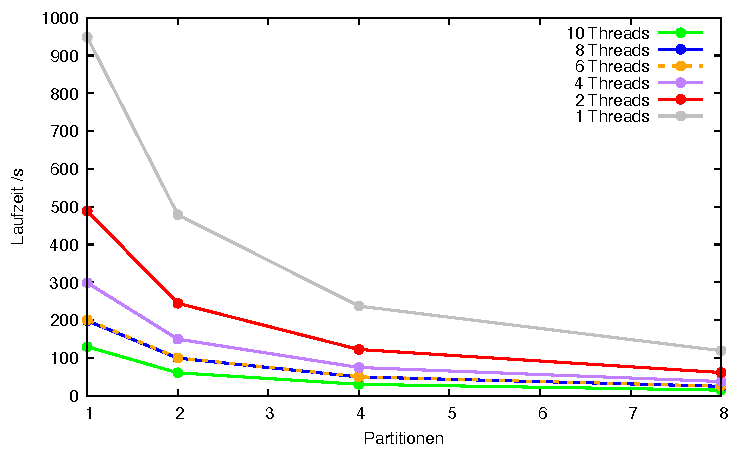
\includegraphics[width=0.8\textwidth]{../results/plots/m1pro/comp_all_threads.pdf}
\caption{Ergebnisse der Leistungstests verglichen nach Thread Anzahl}
\label{fig:m1pro_benchmark_threads}
\end{figure}

\begin{figure}[htbp!]
\centering
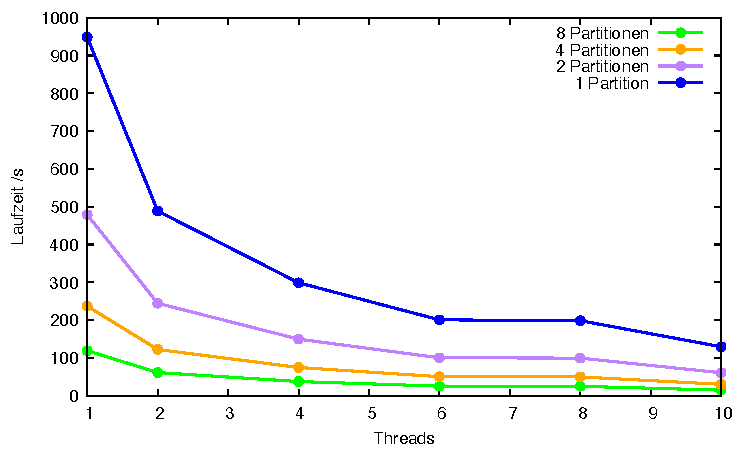
\includegraphics[width=0.8\textwidth]{../results/plots/m1pro/comp_all_partitions.pdf}
\caption{Ergebnisse der Leistungstests verglichen nach Datensatzgröße}
\label{fig:m1pro_benchmark_partitions}
\end{figure}

\subsection{AMD Ryzen 3600XT}

\begin{figure}[htbp!]
\centering
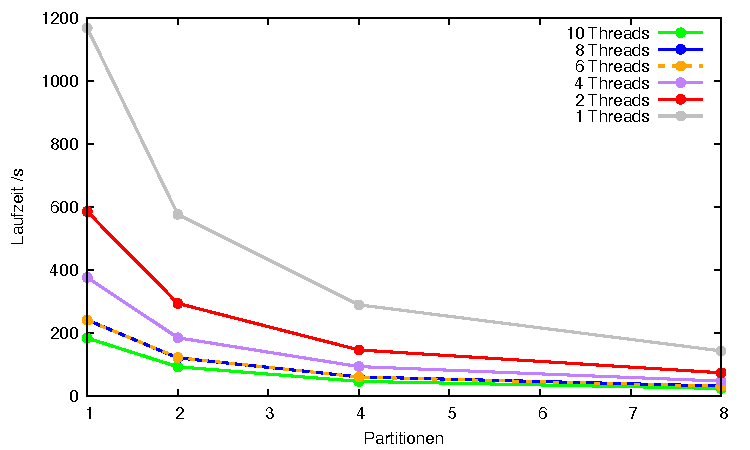
\includegraphics[width=0.8\textwidth]{../results/plots/3600xt/comp_all_threads.pdf}
\caption{Ergebnisse der Leistungstests verglichen nach Thread Anzahl}
\label{fig:ryzen_benchmark_threads}
\end{figure}

\begin{figure}[htbp!]
\centering
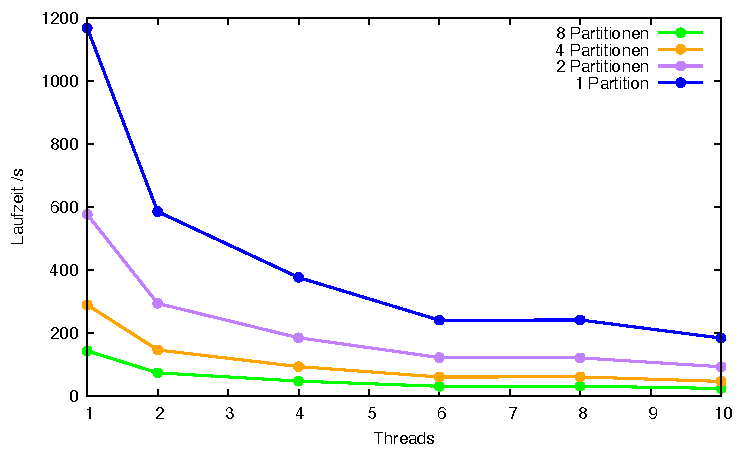
\includegraphics[width=0.8\textwidth]{../results/plots/3600xt/comp_all_partitions.pdf}
\caption{Ergebnisse der Leistungstests verglichen nach Datensatzgröße}
\label{fig:ryzen_benchmark_partitions}
\end{figure}

\subsection{Raspberry Pi 3}

\begin{figure}[htbp!]
\centering
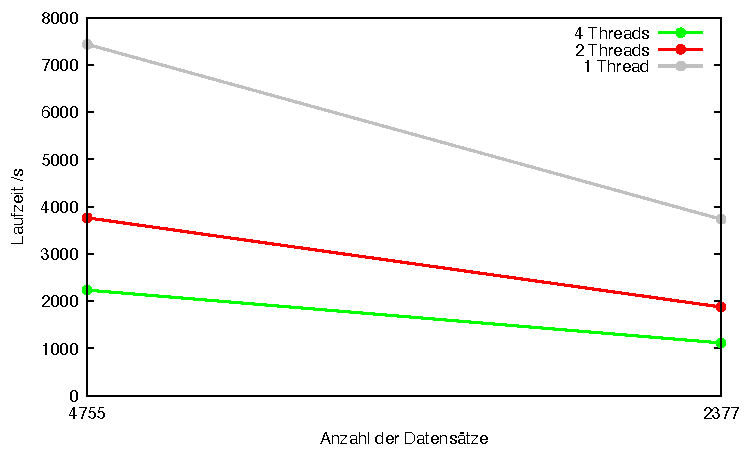
\includegraphics[width=0.8\textwidth]{../results/plots/raspberrypi3/comp_all_threads.pdf}
\caption{Ergebnisse der Leistungstests verglichen nach Thread Anzahl}
\label{fig:raspi_benchmark_threads}
\end{figure}

\begin{figure}[htbp!]
\centering
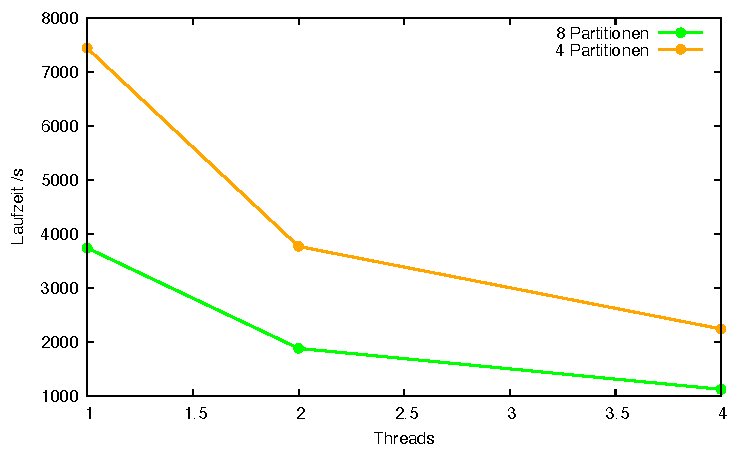
\includegraphics[width=0.8\textwidth]{../results/plots/raspberrypi3/comp_all_partitions.pdf}
\caption{Ergebnisse der Leistungstests verglichen nach Datensatzgröße}
\label{fig:raspi_benchmark_partitions}
\end{figure}

\subsection{Cloud Server}

\section{Auswertung}

\newpage

\chapter{Fazit und Ausblick}
\label{ch:Zusammenfassung}



\begin{appendix}
  \chapter{Programmcode}
\label{Sec:Anhang}


  \clearpage
\end{appendix}

%Falls man die Überschrift des Literaturverzeichnisses
%aendern moechte, geht das durch Verwendung der folgenden Zeile:
%\renewcommand*{\refname}{Literaturverzeichnis}

%\bibliographystyle{plain} % Nummern in eckigen Klammern
%%\bibliographystyle{alpha} % Anfangsbuchstaben Erstautor und Jahr

% Wenn man folgenden Stil verwenden will, dann muss
% \usepackage{harvard} vor \begin{document} aktiviert werden:
%\bibliographystyle{agsm} % (Autoren in runden Klammern)
%\newpage
\clearpage
%\phantomsection % Da sonst falsche Verlinkung im Inhaltsverzeichnis
\printbibliography[heading=bibintoc]    % Ohne Kapitelnummer /-buchstabe
%\printbibliography[heading=bibnumbered]    % Mit Kapitelnummer /-buchstabe
\end{document}
